\documentclass[1p]{elsarticle_modified}
%\bibliographystyle{elsarticle-num}

%\usepackage[colorlinks]{hyperref}
%\usepackage{abbrmath_seonhwa} %\Abb, \Ascr, \Acal ,\Abf, \Afrak
\usepackage{amsfonts}
\usepackage{amssymb}
\usepackage{amsmath}
\usepackage{amsthm}
\usepackage{scalefnt}
\usepackage{amsbsy}
\usepackage{kotex}
\usepackage{caption}
\usepackage{subfig}
\usepackage{color}
\usepackage{graphicx}
\usepackage{xcolor} %% white, black, red, green, blue, cyan, magenta, yellow
\usepackage{float}
\usepackage{setspace}
\usepackage{hyperref}

\usepackage{tikz}
\usetikzlibrary{arrows}

\usepackage{multirow}
\usepackage{array} % fixed length table
\usepackage{hhline}

%%%%%%%%%%%%%%%%%%%%%
\makeatletter
\renewcommand*\env@matrix[1][\arraystretch]{%
	\edef\arraystretch{#1}%
	\hskip -\arraycolsep
	\let\@ifnextchar\new@ifnextchar
	\array{*\c@MaxMatrixCols c}}
\makeatother %https://tex.stackexchange.com/questions/14071/how-can-i-increase-the-line-spacing-in-a-matrix
%%%%%%%%%%%%%%%

\usepackage[normalem]{ulem}

\newcommand{\msout}[1]{\ifmmode\text{\sout{\ensuremath{#1}}}\else\sout{#1}\fi}
%SOURCE: \msout is \stkout macro in https://tex.stackexchange.com/questions/20609/strikeout-in-math-mode

\newcommand{\cancel}[1]{
	\ifmmode
	{\color{red}\msout{#1}}
	\else
	{\color{red}\sout{#1}}
	\fi
}

\newcommand{\add}[1]{
	{\color{blue}\uwave{#1}}
}

\newcommand{\replace}[2]{
	\ifmmode
	{\color{red}\msout{#1}}{\color{blue}\uwave{#2}}
	\else
	{\color{red}\sout{#1}}{\color{blue}\uwave{#2}}
	\fi
}

\newcommand{\Sol}{\mathcal{S}} %segment
\newcommand{\D}{D} %diagram
\newcommand{\A}{\mathcal{A}} %arc


%%%%%%%%%%%%%%%%%%%%%%%%%%%%%5 test

\def\sl{\operatorname{\textup{SL}}(2,\Cbb)}
\def\psl{\operatorname{\textup{PSL}}(2,\Cbb)}
\def\quan{\mkern 1mu \triangleright \mkern 1mu}

\theoremstyle{definition}
\newtheorem{thm}{Theorem}[section]
\newtheorem{prop}[thm]{Proposition}
\newtheorem{lem}[thm]{Lemma}
\newtheorem{ques}[thm]{Question}
\newtheorem{cor}[thm]{Corollary}
\newtheorem{defn}[thm]{Definition}
\newtheorem{exam}[thm]{Example}
\newtheorem{rmk}[thm]{Remark}
\newtheorem{alg}[thm]{Algorithm}

\newcommand{\I}{\sqrt{-1}}
\begin{document}

%\begin{frontmatter}
%
%\title{Boundary parabolic representations of knots up to 8 crossings}
%
%%% Group authors per affiliation:
%\author{Yunhi Cho} 
%\address{Department of Mathematics, University of Seoul, Seoul, Korea}
%\ead{yhcho@uos.ac.kr}
%
%
%\author{Seonhwa Kim} %\fnref{s_kim}}
%\address{Center for Geometry and Physics, Institute for Basic Science, Pohang, 37673, Korea}
%\ead{ryeona17@ibs.re.kr}
%
%\author{Hyuk Kim}
%\address{Department of Mathematical Sciences, Seoul National University, Seoul 08826, Korea}
%\ead{hyukkim@snu.ac.kr}
%
%\author{Seokbeom Yoon}
%\address{Department of Mathematical Sciences, Seoul National University, Seoul, 08826,  Korea}
%\ead{sbyoon15@snu.ac.kr}
%
%\begin{abstract}
%We find all boundary parabolic representation of knots up to 8 crossings.
%
%\end{abstract}
%\begin{keyword}
%    \MSC[2010] 57M25 
%\end{keyword}
%
%\end{frontmatter}

%\linenumbers
%\tableofcontents
%
\newcommand\colored[1]{\textcolor{white}{\rule[-0.35ex]{0.8em}{1.4ex}}\kern-0.8em\color{red} #1}%
%\newcommand\colored[1]{\textcolor{white}{ #1}\kern-2.17ex	\textcolor{white}{ #1}\kern-1.81ex	\textcolor{white}{ #1}\kern-2.15ex\color{red}#1	}

{\Large $\underline{11n_{161}~(K11n_{161})}$}

\setlength{\tabcolsep}{10pt}
\renewcommand{\arraystretch}{1.6}
\vspace{1cm}\begin{tabular}{m{100pt}>{\centering\arraybackslash}m{274pt}}
\multirow{5}{120pt}{
	\centering
	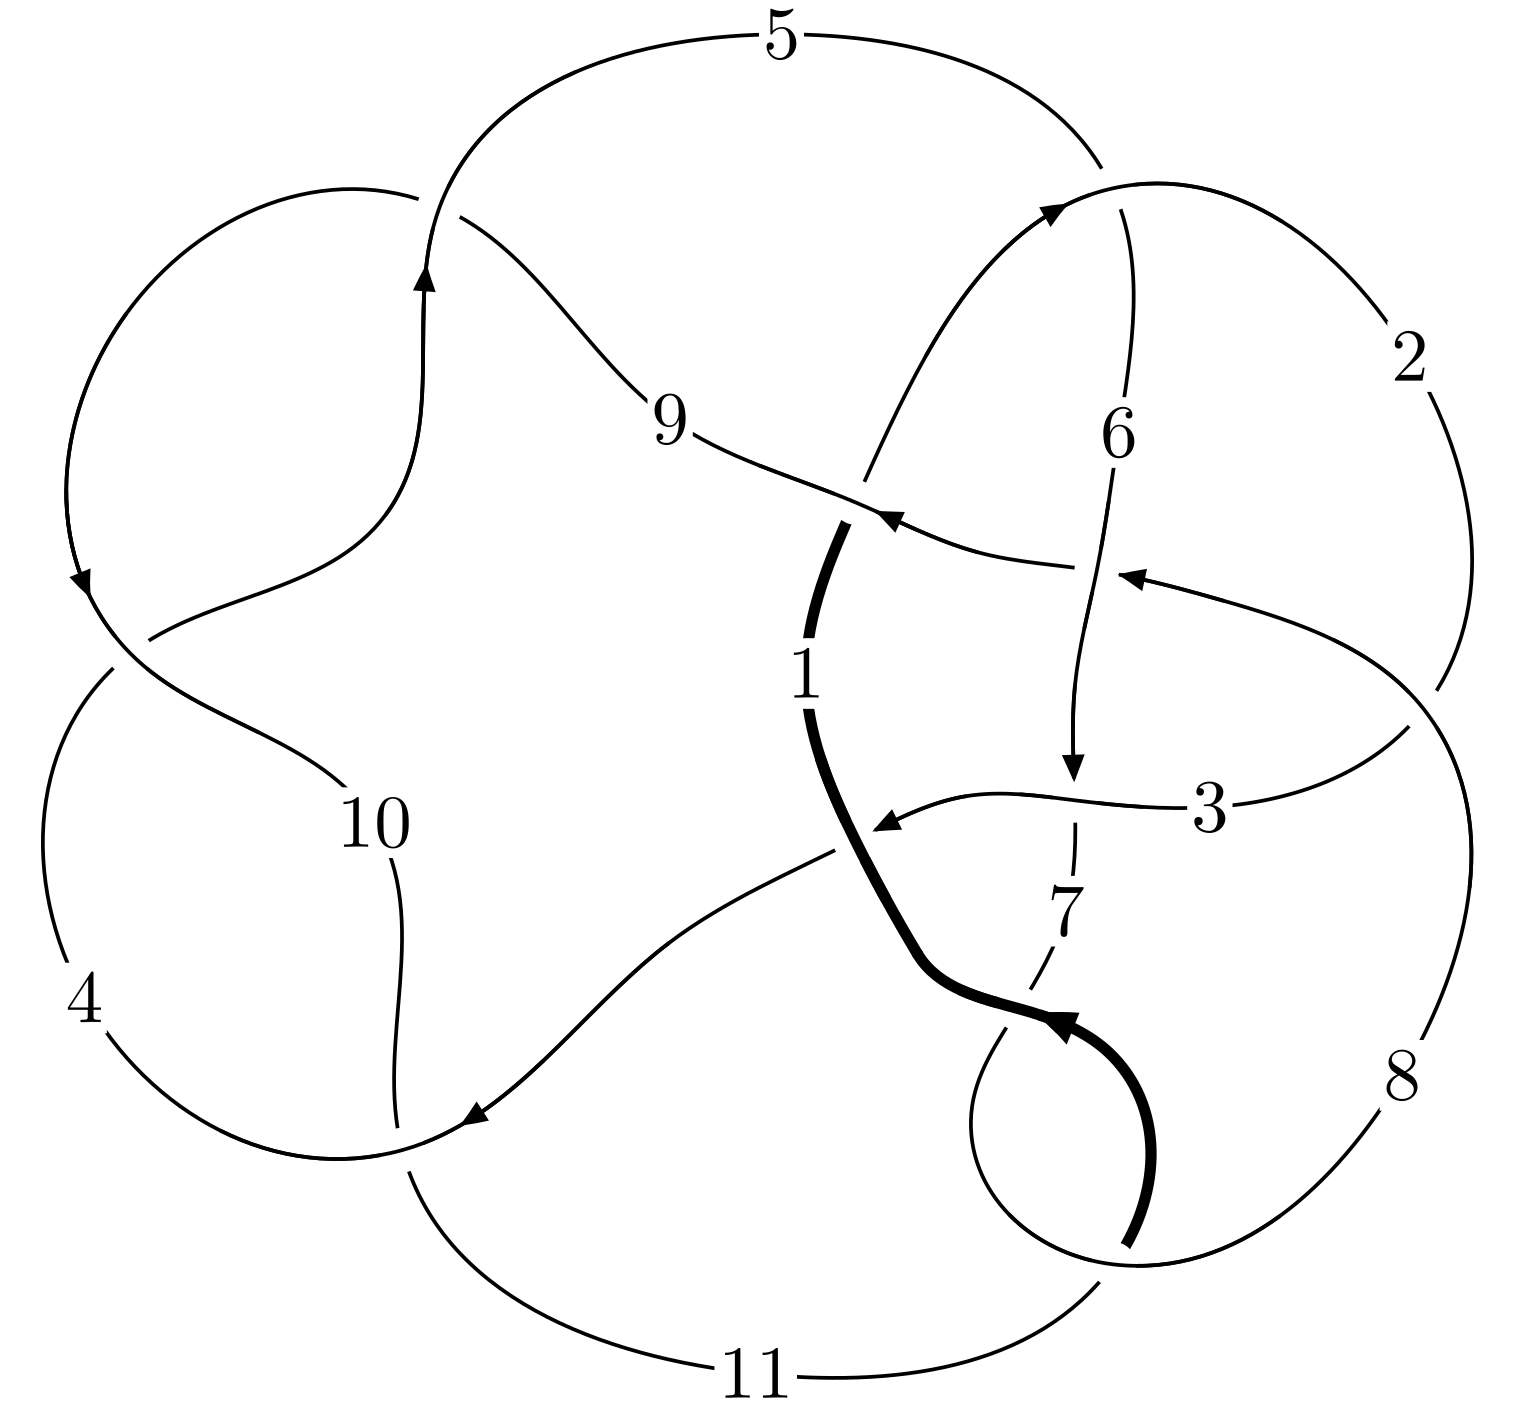
\includegraphics[width=112pt]{../../../GIT/diagram.site/Diagrams/png/777_11n_161.png}\\
\ \ \ A knot diagram\footnotemark}&
\allowdisplaybreaks
\textbf{Linearized knot diagam} \\
\cline{2-2}
 &
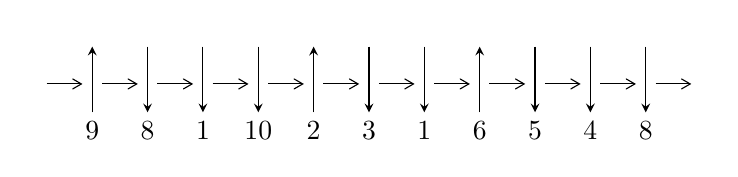
\begin{tikzpicture}[x=20pt, y=17pt]
	% nodes
	\node (C0) at (0, 0) {};
	\node (C1) at (1, 0) {};
	\node (C1U) at (1, +1) {};
	\node (C1D) at (1, -1) {9};

	\node (C2) at (2, 0) {};
	\node (C2U) at (2, +1) {};
	\node (C2D) at (2, -1) {8};

	\node (C3) at (3, 0) {};
	\node (C3U) at (3, +1) {};
	\node (C3D) at (3, -1) {1};

	\node (C4) at (4, 0) {};
	\node (C4U) at (4, +1) {};
	\node (C4D) at (4, -1) {10};

	\node (C5) at (5, 0) {};
	\node (C5U) at (5, +1) {};
	\node (C5D) at (5, -1) {2};

	\node (C6) at (6, 0) {};
	\node (C6U) at (6, +1) {};
	\node (C6D) at (6, -1) {3};

	\node (C7) at (7, 0) {};
	\node (C7U) at (7, +1) {};
	\node (C7D) at (7, -1) {1};

	\node (C8) at (8, 0) {};
	\node (C8U) at (8, +1) {};
	\node (C8D) at (8, -1) {6};

	\node (C9) at (9, 0) {};
	\node (C9U) at (9, +1) {};
	\node (C9D) at (9, -1) {5};

	\node (C10) at (10, 0) {};
	\node (C10U) at (10, +1) {};
	\node (C10D) at (10, -1) {4};

	\node (C11) at (11, 0) {};
	\node (C11U) at (11, +1) {};
	\node (C11D) at (11, -1) {8};
	\node (C12) at (12, 0) {};

	% arrows
	\draw[->,>={angle 60}]
	(C0) edge (C1) (C1) edge (C2) (C2) edge (C3) (C3) edge (C4) (C4) edge (C5) (C5) edge (C6) (C6) edge (C7) (C7) edge (C8) (C8) edge (C9) (C9) edge (C10) (C10) edge (C11) (C11) edge (C12) ;	\draw[->,>=stealth]
	(C1D) edge (C1U) (C2U) edge (C2D) (C3U) edge (C3D) (C4U) edge (C4D) (C5D) edge (C5U) (C6U) edge (C6D) (C7U) edge (C7D) (C8D) edge (C8U) (C9U) edge (C9D) (C10U) edge (C10D) (C11U) edge (C11D) ;
	\end{tikzpicture} \\
\hhline{~~} \\& 
\textbf{Solving Sequence} \\ \cline{2-2} 
 &
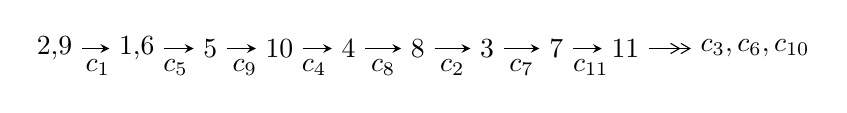
\begin{tikzpicture}[x=25pt, y=7pt]
	% node
	\node (A0) at (-1/8, 0) {2,9};
	\node (A1) at (17/16, 0) {1,6};
	\node (A2) at (17/8, 0) {5};
	\node (A3) at (25/8, 0) {10};
	\node (A4) at (33/8, 0) {4};
	\node (A5) at (41/8, 0) {8};
	\node (A6) at (49/8, 0) {3};
	\node (A7) at (57/8, 0) {7};
	\node (A8) at (65/8, 0) {11};
	\node (C1) at (1/2, -1) {$c_{1}$};
	\node (C2) at (13/8, -1) {$c_{5}$};
	\node (C3) at (21/8, -1) {$c_{9}$};
	\node (C4) at (29/8, -1) {$c_{4}$};
	\node (C5) at (37/8, -1) {$c_{8}$};
	\node (C6) at (45/8, -1) {$c_{2}$};
	\node (C7) at (53/8, -1) {$c_{7}$};
	\node (C8) at (61/8, -1) {$c_{11}$};
	\node (A9) at (10, 0) {$c_{3},c_{6},c_{10}$};

	% edge
	\draw[->,>=stealth]	
	(A0) edge (A1) (A1) edge (A2) (A2) edge (A3) (A3) edge (A4) (A4) edge (A5) (A5) edge (A6) (A6) edge (A7) (A7) edge (A8) ;
	\draw[->>,>={angle 60}]	
	(A8) edge (A9);
\end{tikzpicture} \\ 

\end{tabular} \\

\footnotetext{
The image of knot diagram is generated by the software ``\textbf{Draw programme}" developed by Andrew Bartholomew(\url{http://www.layer8.co.uk/maths/draw/index.htm\#Running-draw}), where we modified some parts for our purpose(\url{https://github.com/CATsTAILs/LinksPainter}).
}\phantom \\ \newline 
\centering \textbf{Ideals for irreducible components\footnotemark of $X_{\text{par}}$} 
 
\begin{align*}
I^u_{1}&=\langle 
b- u,\;-32825 u^{16}-78351 u^{15}+\cdots+149349 a+108694,\\
\phantom{I^u_{1}}&\phantom{= \langle  }u^{17}+u^{16}- u^{15}- u^{14}+9 u^{13}+7 u^{12}-5 u^{11}-2 u^{10}+18 u^9+12 u^8-4 u^7-5 u^6+5 u^5- u^4- u^3- u^2+u-1\rangle \\
I^u_{2}&=\langle 
1.70203\times10^{30} u^{23}+4.57303\times10^{30} u^{22}+\cdots+8.77268\times10^{30} b+5.47196\times10^{31},\\
\phantom{I^u_{2}}&\phantom{= \langle  }-6.45612\times10^{27} u^{23}-1.61756\times10^{28} u^{22}+\cdots+5.13568\times10^{28} a-1.36907\times10^{29},\\
\phantom{I^u_{2}}&\phantom{= \langle  }u^{24}+3 u^{23}+\cdots+46 u+11\rangle \\
I^u_{3}&=\langle 
b+u,\;-14 u^9- u^8+16 u^7-3 u^6-69 u^5+26 u^4+25 u^3-21 u^2+5 a-20 u-12,\\
\phantom{I^u_{3}}&\phantom{= \langle  }u^{10}+u^9- u^8- u^7+5 u^6+3 u^5-3 u^4- u^3+3 u^2+3 u+1\rangle \\
\\
\end{align*}
\raggedright * 3 irreducible components of $\dim_{\mathbb{C}}=0$, with total 51 representations.\\
\footnotetext{All coefficients of polynomials are rational numbers. But the coefficients are sometimes approximated in decimal forms when there is not enough margin.}
\newpage
\renewcommand{\arraystretch}{1}
\centering \section*{I. $I^u_{1}= \langle b- u,\;-3.28\times10^{4} u^{16}-7.84\times10^{4} u^{15}+\cdots+1.49\times10^{5} a+1.09\times10^{5},\;u^{17}+u^{16}+\cdots+u-1 \rangle$}
\flushleft \textbf{(i) Arc colorings}\\
\begin{tabular}{m{7pt} m{180pt} m{7pt} m{180pt} }
\flushright $a_{2}=$&$\begin{pmatrix}1\\0\end{pmatrix}$ \\
\flushright $a_{9}=$&$\begin{pmatrix}0\\u\end{pmatrix}$ \\
\flushright $a_{1}=$&$\begin{pmatrix}1\\u^2\end{pmatrix}$ \\
\flushright $a_{6}=$&$\begin{pmatrix}0.219787 u^{16}+0.524617 u^{15}+\cdots+1.20532 u-0.727785\\u\end{pmatrix}$ \\
\flushright $a_{5}=$&$\begin{pmatrix}0.219787 u^{16}+0.524617 u^{15}+\cdots+0.205324 u-0.727785\\u\end{pmatrix}$ \\
\flushright $a_{10}=$&$\begin{pmatrix}0.966327 u^{16}+1.11448 u^{15}+\cdots-2.99444 u+1.19912\\-0.0803353 u^{16}-0.516903 u^{15}+\cdots+1.08504 u-0.304830\end{pmatrix}$ \\
\flushright $a_{4}=$&$\begin{pmatrix}0.265559 u^{16}+0.586479 u^{15}+\cdots+3.63417 u+1.42934\\-0.537426 u^{16}-0.452303 u^{15}+\cdots+0.266865 u-0.452979\end{pmatrix}$ \\
\flushright $a_{8}=$&$\begin{pmatrix}0.805657 u^{16}+0.0806701 u^{15}+\cdots-2.82436 u+0.589458\\-0.0803353 u^{16}-0.516903 u^{15}+\cdots+1.08504 u-0.304830\end{pmatrix}$ \\
\flushright $a_{3}=$&$\begin{pmatrix}0.567001 u^{16}+0.839992 u^{15}+\cdots+3.95640 u+0.655438\\-0.544229 u^{16}-0.276594 u^{15}+\cdots+0.616234 u-0.500907\end{pmatrix}$ \\
\flushright $a_{7}=$&$\begin{pmatrix}0.385085 u^{16}-0.447562 u^{15}+\cdots-3.26996 u+1.00962\\0.245726 u^{16}-0.325151 u^{15}+\cdots+0.772131 u-0.412490\end{pmatrix}$ \\
\flushright $a_{11}=$&$\begin{pmatrix}0.175562 u^{16}+1.94315 u^{15}+\cdots+2.59534 u+1.27888\\-0.301442 u^{16}-0.253514 u^{15}+\cdots-0.322225 u+0.773899\end{pmatrix}$\\ \flushright $a_{11}=$&$\begin{pmatrix}0.175562 u^{16}+1.94315 u^{15}+\cdots+2.59534 u+1.27888\\-0.301442 u^{16}-0.253514 u^{15}+\cdots-0.322225 u+0.773899\end{pmatrix}$\\&\end{tabular}
\flushleft \textbf{(ii) Obstruction class $= -1$}\\~\\
\flushleft \textbf{(iii) Cusp Shapes $= \frac{163298}{149349} u^{16}+\frac{580790}{149349} u^{15}+\cdots+\frac{328192}{149349} u-\frac{306609}{49783}$}\\~\\
\newpage\renewcommand{\arraystretch}{1}
\flushleft \textbf{(iv) u-Polynomials at the component}\newline \\
\begin{tabular}{m{50pt}|m{274pt}}
Crossings & \hspace{64pt}u-Polynomials at each crossing \\
\hline $$\begin{aligned}c_{1},c_{5}\end{aligned}$$&$\begin{aligned}
&u^{17}- u^{16}+\cdots+u+1
\end{aligned}$\\
\hline $$\begin{aligned}c_{2}\end{aligned}$$&$\begin{aligned}
&u^{17}-2 u^{15}+\cdots- u-2
\end{aligned}$\\
\hline $$\begin{aligned}c_{3}\end{aligned}$$&$\begin{aligned}
&u^{17}-14 u^{16}+\cdots-32 u-64
\end{aligned}$\\
\hline $$\begin{aligned}c_{4},c_{9},c_{10}\end{aligned}$$&$\begin{aligned}
&u^{17}+9 u^{16}+\cdots+144 u+16
\end{aligned}$\\
\hline $$\begin{aligned}c_{6},c_{7},c_{11}\end{aligned}$$&$\begin{aligned}
&u^{17}+u^{16}+\cdots+u+1
\end{aligned}$\\
\hline $$\begin{aligned}c_{8}\end{aligned}$$&$\begin{aligned}
&u^{17}+12 u^{16}+\cdots+64 u+8
\end{aligned}$\\
\hline
\end{tabular}\\~\\
\newpage\renewcommand{\arraystretch}{1}
\flushleft \textbf{(v) Riley Polynomials at the component}\newline \\
\begin{tabular}{m{50pt}|m{274pt}}
Crossings & \hspace{64pt}Riley Polynomials at each crossing \\
\hline $$\begin{aligned}c_{1},c_{5}\end{aligned}$$&$\begin{aligned}
&y^{17}-3 y^{16}+\cdots- y-1
\end{aligned}$\\
\hline $$\begin{aligned}c_{2}\end{aligned}$$&$\begin{aligned}
&y^{17}-4 y^{16}+\cdots+29 y-4
\end{aligned}$\\
\hline $$\begin{aligned}c_{3}\end{aligned}$$&$\begin{aligned}
&y^{17}-14 y^{16}+\cdots+50688 y-4096
\end{aligned}$\\
\hline $$\begin{aligned}c_{4},c_{9},c_{10}\end{aligned}$$&$\begin{aligned}
&y^{17}+15 y^{16}+\cdots-128 y-256
\end{aligned}$\\
\hline $$\begin{aligned}c_{6},c_{7},c_{11}\end{aligned}$$&$\begin{aligned}
&y^{17}-23 y^{16}+\cdots+9 y-1
\end{aligned}$\\
\hline $$\begin{aligned}c_{8}\end{aligned}$$&$\begin{aligned}
&y^{17}+4 y^{16}+\cdots-608 y-64
\end{aligned}$\\
\hline
\end{tabular}\\~\\
\newpage\flushleft \textbf{(vi) Complex Volumes and Cusp Shapes}
$$\begin{array}{c|c|c}  
\text{Solutions to }I^u_{1}& \I (\text{vol} + \sqrt{-1}CS) & \text{Cusp shape}\\
 \hline 
\begin{aligned}
u &= -0.736595 + 0.759560 I \\
a &= -0.631113 + 0.062721 I \\
b &= -0.736595 + 0.759560 I\end{aligned}
 & -0.05757 - 2.36290 I & -6.52154 + 3.94257 I \\ \hline\begin{aligned}
u &= -0.736595 - 0.759560 I \\
a &= -0.631113 - 0.062721 I \\
b &= -0.736595 - 0.759560 I\end{aligned}
 & -0.05757 + 2.36290 I & -6.52154 - 3.94257 I \\ \hline\begin{aligned}
u &= -1.008910 + 0.431442 I \\
a &= -0.889354 - 0.979858 I \\
b &= -1.008910 + 0.431442 I\end{aligned}
 & \phantom{-}1.14436 - 6.14847 I & -1.51565 + 5.18000 I \\ \hline\begin{aligned}
u &= -1.008910 - 0.431442 I \\
a &= -0.889354 + 0.979858 I \\
b &= -1.008910 - 0.431442 I\end{aligned}
 & \phantom{-}1.14436 + 6.14847 I & -1.51565 - 5.18000 I \\ \hline\begin{aligned}
u &= -0.534388 + 0.570811 I \\
a &= -2.28268 + 0.49285 I \\
b &= -0.534388 + 0.570811 I\end{aligned}
 & -5.66005 - 1.97491 I & -5.96248 + 6.00520 I \\ \hline\begin{aligned}
u &= -0.534388 - 0.570811 I \\
a &= -2.28268 - 0.49285 I \\
b &= -0.534388 - 0.570811 I\end{aligned}
 & -5.66005 + 1.97491 I & -5.96248 - 6.00520 I \\ \hline\begin{aligned}
u &= \phantom{-}0.700751\phantom{ +0.000000I} \\
a &= \phantom{-}2.48391\phantom{ +0.000000I} \\
b &= \phantom{-}0.700751\phantom{ +0.000000I}\end{aligned}
 & -3.84845\phantom{ +0.000000I} & \phantom{-}2.74050\phantom{ +0.000000I} \\ \hline\begin{aligned}
u &= \phantom{-}0.902645 + 0.958889 I \\
a &= \phantom{-}1.194590 + 0.162669 I \\
b &= \phantom{-}0.902645 + 0.958889 I\end{aligned}
 & -6.98471 + 8.59095 I & -7.08514 - 6.35872 I \\ \hline\begin{aligned}
u &= \phantom{-}0.902645 - 0.958889 I \\
a &= \phantom{-}1.194590 - 0.162669 I \\
b &= \phantom{-}0.902645 - 0.958889 I\end{aligned}
 & -6.98471 - 8.59095 I & -7.08514 + 6.35872 I \\ \hline\begin{aligned}
u &= \phantom{-}0.482184 + 0.448786 I \\
a &= -1.16928 - 1.33243 I \\
b &= \phantom{-}0.482184 + 0.448786 I\end{aligned}
 & \phantom{-}5.38217 + 1.40715 I & -2.06078 - 4.92367 I\\
 \hline 
 \end{array}$$\newpage$$\begin{array}{c|c|c}  
\text{Solutions to }I^u_{1}& \I (\text{vol} + \sqrt{-1}CS) & \text{Cusp shape}\\
 \hline 
\begin{aligned}
u &= \phantom{-}0.482184 - 0.448786 I \\
a &= -1.16928 + 1.33243 I \\
b &= \phantom{-}0.482184 - 0.448786 I\end{aligned}
 & \phantom{-}5.38217 - 1.40715 I & -2.06078 + 4.92367 I \\ \hline\begin{aligned}
u &= \phantom{-}0.175989 + 0.585685 I \\
a &= \phantom{-}0.864699 + 0.113620 I \\
b &= \phantom{-}0.175989 + 0.585685 I\end{aligned}
 & -0.850953 - 0.696665 I & -8.07292 + 4.89884 I \\ \hline\begin{aligned}
u &= \phantom{-}0.175989 - 0.585685 I \\
a &= \phantom{-}0.864699 - 0.113620 I \\
b &= \phantom{-}0.175989 - 0.585685 I\end{aligned}
 & -0.850953 + 0.696665 I & -8.07292 - 4.89884 I \\ \hline\begin{aligned}
u &= \phantom{-}1.14438 + 0.95543 I \\
a &= \phantom{-}0.540728 + 0.095251 I \\
b &= \phantom{-}1.14438 + 0.95543 I\end{aligned}
 & \phantom{-}7.19647 + 4.49345 I & -5.42758 + 0.47721 I \\ \hline\begin{aligned}
u &= \phantom{-}1.14438 - 0.95543 I \\
a &= \phantom{-}0.540728 - 0.095251 I \\
b &= \phantom{-}1.14438 - 0.95543 I\end{aligned}
 & \phantom{-}7.19647 - 4.49345 I & -5.42758 - 0.47721 I \\ \hline\begin{aligned}
u &= -1.27568 + 1.06823 I \\
a &= -0.869544 + 0.210846 I \\
b &= -1.27568 + 1.06823 I\end{aligned}
 & -0.71290 - 13.72760 I & -3.72416 + 7.05259 I \\ \hline\begin{aligned}
u &= -1.27568 - 1.06823 I \\
a &= -0.869544 - 0.210846 I \\
b &= -1.27568 - 1.06823 I\end{aligned}
 & -0.71290 + 13.72760 I & -3.72416 - 7.05259 I\\
 \hline 
 \end{array}$$\newpage\newpage\renewcommand{\arraystretch}{1}
\centering \section*{II. $I^u_{2}= \langle 1.70\times10^{30} u^{23}+4.57\times10^{30} u^{22}+\cdots+8.77\times10^{30} b+5.47\times10^{31},\;-6.46\times10^{27} u^{23}-1.62\times10^{28} u^{22}+\cdots+5.14\times10^{28} a-1.37\times10^{29},\;u^{24}+3 u^{23}+\cdots+46 u+11 \rangle$}
\flushleft \textbf{(i) Arc colorings}\\
\begin{tabular}{m{7pt} m{180pt} m{7pt} m{180pt} }
\flushright $a_{2}=$&$\begin{pmatrix}1\\0\end{pmatrix}$ \\
\flushright $a_{9}=$&$\begin{pmatrix}0\\u\end{pmatrix}$ \\
\flushright $a_{1}=$&$\begin{pmatrix}1\\u^2\end{pmatrix}$ \\
\flushright $a_{6}=$&$\begin{pmatrix}0.125711 u^{23}+0.314966 u^{22}+\cdots+7.79270 u+2.66581\\-0.194014 u^{23}-0.521280 u^{22}+\cdots-10.4641 u-6.23750\end{pmatrix}$ \\
\flushright $a_{5}=$&$\begin{pmatrix}0.319725 u^{23}+0.836246 u^{22}+\cdots+18.2568 u+8.90330\\-0.194014 u^{23}-0.521280 u^{22}+\cdots-10.4641 u-6.23750\end{pmatrix}$ \\
\flushright $a_{10}=$&$\begin{pmatrix}-0.0116621 u^{23}-0.0806554 u^{22}+\cdots+4.00812 u-3.44719\\-0.175665 u^{23}-0.437895 u^{22}+\cdots-9.21681 u-2.60383\end{pmatrix}$ \\
\flushright $a_{4}=$&$\begin{pmatrix}-0.240478 u^{23}-0.644174 u^{22}+\cdots-11.8851 u-8.16867\\0.0316958 u^{23}+0.103215 u^{22}+\cdots+0.735566 u+2.15396\end{pmatrix}$ \\
\flushright $a_{8}=$&$\begin{pmatrix}-0.190587 u^{23}-0.510517 u^{22}+\cdots-7.93355 u-4.80896\\-0.00326046 u^{23}+0.00803404 u^{22}+\cdots-0.724864 u+1.24206\end{pmatrix}$ \\
\flushright $a_{3}=$&$\begin{pmatrix}-0.190071 u^{23}-0.496722 u^{22}+\cdots-10.2408 u-5.16485\\0.0231595 u^{23}+0.0870786 u^{22}+\cdots+0.354516 u+2.19543\end{pmatrix}$ \\
\flushright $a_{7}=$&$\begin{pmatrix}-0.148842 u^{23}-0.367537 u^{22}+\cdots-7.93760 u-2.89321\\-0.0152103 u^{23}-0.0113006 u^{22}+\cdots-2.00024 u+1.04689\end{pmatrix}$ \\
\flushright $a_{11}=$&$\begin{pmatrix}0.240478 u^{23}+0.644174 u^{22}+\cdots+11.8851 u+8.16867\\-0.0504074 u^{23}-0.147452 u^{22}+\cdots-1.64431 u-3.00383\end{pmatrix}$\\ \flushright $a_{11}=$&$\begin{pmatrix}0.240478 u^{23}+0.644174 u^{22}+\cdots+11.8851 u+8.16867\\-0.0504074 u^{23}-0.147452 u^{22}+\cdots-1.64431 u-3.00383\end{pmatrix}$\\&\end{tabular}
\flushleft \textbf{(ii) Obstruction class $= -1$}\\~\\
\flushleft \textbf{(iii) Cusp Shapes $= 0.802694 u^{23}+2.06436 u^{22}+\cdots+39.8732 u+14.4982$}\\~\\
\newpage\renewcommand{\arraystretch}{1}
\flushleft \textbf{(iv) u-Polynomials at the component}\newline \\
\begin{tabular}{m{50pt}|m{274pt}}
Crossings & \hspace{64pt}u-Polynomials at each crossing \\
\hline $$\begin{aligned}c_{1},c_{5}\end{aligned}$$&$\begin{aligned}
&u^{24}-3 u^{23}+\cdots-46 u+11
\end{aligned}$\\
\hline $$\begin{aligned}c_{2}\end{aligned}$$&$\begin{aligned}
&u^{24}- u^{23}+\cdots-178 u+59
\end{aligned}$\\
\hline $$\begin{aligned}c_{3}\end{aligned}$$&$\begin{aligned}
&(u^4+3 u^3+u^2-2 u+1)^6
\end{aligned}$\\
\hline $$\begin{aligned}c_{4},c_{9},c_{10}\end{aligned}$$&$\begin{aligned}
&(u^3- u^2+2 u-1)^8
\end{aligned}$\\
\hline $$\begin{aligned}c_{6},c_{7},c_{11}\end{aligned}$$&$\begin{aligned}
&u^{24}- u^{23}+\cdots-568 u+89
\end{aligned}$\\
\hline $$\begin{aligned}c_{8}\end{aligned}$$&$\begin{aligned}
&(u^4- u^3+u^2+1)^6
\end{aligned}$\\
\hline
\end{tabular}\\~\\
\newpage\renewcommand{\arraystretch}{1}
\flushleft \textbf{(v) Riley Polynomials at the component}\newline \\
\begin{tabular}{m{50pt}|m{274pt}}
Crossings & \hspace{64pt}Riley Polynomials at each crossing \\
\hline $$\begin{aligned}c_{1},c_{5}\end{aligned}$$&$\begin{aligned}
&y^{24}-5 y^{23}+\cdots-1544 y+121
\end{aligned}$\\
\hline $$\begin{aligned}c_{2}\end{aligned}$$&$\begin{aligned}
&y^{24}-9 y^{23}+\cdots-77232 y+3481
\end{aligned}$\\
\hline $$\begin{aligned}c_{3}\end{aligned}$$&$\begin{aligned}
&(y^4-7 y^3+15 y^2-2 y+1)^6
\end{aligned}$\\
\hline $$\begin{aligned}c_{4},c_{9},c_{10}\end{aligned}$$&$\begin{aligned}
&(y^3+3 y^2+2 y-1)^8
\end{aligned}$\\
\hline $$\begin{aligned}c_{6},c_{7},c_{11}\end{aligned}$$&$\begin{aligned}
&y^{24}-21 y^{23}+\cdots-204788 y+7921
\end{aligned}$\\
\hline $$\begin{aligned}c_{8}\end{aligned}$$&$\begin{aligned}
&(y^4+y^3+3 y^2+2 y+1)^6
\end{aligned}$\\
\hline
\end{tabular}\\~\\
\newpage\flushleft \textbf{(vi) Complex Volumes and Cusp Shapes}
$$\begin{array}{c|c|c}  
\text{Solutions to }I^u_{2}& \I (\text{vol} + \sqrt{-1}CS) & \text{Cusp shape}\\
 \hline 
\begin{aligned}
u &= -0.726600 + 0.525022 I \\
a &= \phantom{-}0.174808 + 1.380500 I \\
b &= \phantom{-}0.834345 + 0.058079 I\end{aligned}
 & \phantom{-}4.88007 + 0.33584 I & -2.66351 + 0.41465 I \\ \hline\begin{aligned}
u &= -0.726600 - 0.525022 I \\
a &= \phantom{-}0.174808 - 1.380500 I \\
b &= \phantom{-}0.834345 - 0.058079 I\end{aligned}
 & \phantom{-}4.88007 - 0.33584 I & -2.66351 - 0.41465 I \\ \hline\begin{aligned}
u &= \phantom{-}0.834345 + 0.058079 I \\
a &= -1.09167 - 1.01623 I \\
b &= -0.726600 + 0.525022 I\end{aligned}
 & \phantom{-}4.88007 + 0.33584 I & -2.66351 + 0.41465 I \\ \hline\begin{aligned}
u &= \phantom{-}0.834345 - 0.058079 I \\
a &= -1.09167 + 1.01623 I \\
b &= -0.726600 - 0.525022 I\end{aligned}
 & \phantom{-}4.88007 - 0.33584 I & -2.66351 - 0.41465 I \\ \hline\begin{aligned}
u &= -0.951037 + 0.715358 I \\
a &= \phantom{-}1.032340 - 0.181700 I \\
b &= \phantom{-}0.649666 - 0.469539 I\end{aligned}
 & \phantom{-}0.74248 - 3.16396 I & -9.19277 + 2.56480 I \\ \hline\begin{aligned}
u &= -0.951037 - 0.715358 I \\
a &= \phantom{-}1.032340 + 0.181700 I \\
b &= \phantom{-}0.649666 + 0.469539 I\end{aligned}
 & \phantom{-}0.74248 + 3.16396 I & -9.19277 - 2.56480 I \\ \hline\begin{aligned}
u &= \phantom{-}0.649666 + 0.469539 I \\
a &= -1.52720 - 0.29894 I \\
b &= -0.951037 - 0.715358 I\end{aligned}
 & \phantom{-}0.74248 + 3.16396 I & -9.19277 - 2.56480 I \\ \hline\begin{aligned}
u &= \phantom{-}0.649666 - 0.469539 I \\
a &= -1.52720 + 0.29894 I \\
b &= -0.951037 + 0.715358 I\end{aligned}
 & \phantom{-}0.74248 - 3.16396 I & -9.19277 + 2.56480 I \\ \hline\begin{aligned}
u &= -0.238976 + 1.192720 I \\
a &= -0.637456 - 0.167240 I \\
b &= -1.72582 - 0.12950 I\end{aligned}
 & -2.12168 + 1.41302 I & -6.31698 + 1.92930 I \\ \hline\begin{aligned}
u &= -0.238976 - 1.192720 I \\
a &= -0.637456 + 0.167240 I \\
b &= -1.72582 + 0.12950 I\end{aligned}
 & -2.12168 - 1.41302 I & -6.31698 - 1.92930 I\\
 \hline 
 \end{array}$$\newpage$$\begin{array}{c|c|c}  
\text{Solutions to }I^u_{2}& \I (\text{vol} + \sqrt{-1}CS) & \text{Cusp shape}\\
 \hline 
\begin{aligned}
u &= \phantom{-}0.168821 + 0.703789 I \\
a &= \phantom{-}1.081210 - 0.240521 I \\
b &= \phantom{-}1.26487 - 1.00614 I\end{aligned}
 & -6.25926 + 1.41510 I & -12.84625 - 4.90874 I \\ \hline\begin{aligned}
u &= \phantom{-}0.168821 - 0.703789 I \\
a &= \phantom{-}1.081210 + 0.240521 I \\
b &= \phantom{-}1.26487 + 1.00614 I\end{aligned}
 & -6.25926 - 1.41510 I & -12.84625 + 4.90874 I \\ \hline\begin{aligned}
u &= -0.939501 + 0.901901 I \\
a &= \phantom{-}0.956419 - 0.051833 I \\
b &= \phantom{-}1.53236 - 0.89026 I\end{aligned}
 & \phantom{-}4.88007 - 5.99209 I & -2.66351 + 5.54425 I \\ \hline\begin{aligned}
u &= -0.939501 - 0.901901 I \\
a &= \phantom{-}0.956419 + 0.051833 I \\
b &= \phantom{-}1.53236 + 0.89026 I\end{aligned}
 & \phantom{-}4.88007 + 5.99209 I & -2.66351 - 5.54425 I \\ \hline\begin{aligned}
u &= -0.369838 + 0.105617 I \\
a &= -1.39380 + 1.54969 I \\
b &= -0.99828 - 1.87172 I\end{aligned}
 & -2.12168 - 4.24323 I & -6.31698 + 7.88819 I \\ \hline\begin{aligned}
u &= -0.369838 - 0.105617 I \\
a &= -1.39380 - 1.54969 I \\
b &= -0.99828 + 1.87172 I\end{aligned}
 & -2.12168 + 4.24323 I & -6.31698 - 7.88819 I \\ \hline\begin{aligned}
u &= \phantom{-}1.26487 + 1.00614 I \\
a &= -0.107103 - 0.484305 I \\
b &= \phantom{-}0.168821 - 0.703789 I\end{aligned}
 & -6.25926 - 1.41510 I & -12.84625 + 4.90874 I \\ \hline\begin{aligned}
u &= \phantom{-}1.26487 - 1.00614 I \\
a &= -0.107103 + 0.484305 I \\
b &= \phantom{-}0.168821 + 0.703789 I\end{aligned}
 & -6.25926 + 1.41510 I & -12.84625 - 4.90874 I \\ \hline\begin{aligned}
u &= -1.72582 + 0.12950 I \\
a &= -0.171564 - 0.430263 I \\
b &= -0.238976 - 1.192720 I\end{aligned}
 & -2.12168 - 1.41302 I & -6.31698 - 1.92930 I \\ \hline\begin{aligned}
u &= -1.72582 - 0.12950 I \\
a &= -0.171564 + 0.430263 I \\
b &= -0.238976 + 1.192720 I\end{aligned}
 & -2.12168 + 1.41302 I & -6.31698 + 1.92930 I\\
 \hline 
 \end{array}$$\newpage$$\begin{array}{c|c|c}  
\text{Solutions to }I^u_{2}& \I (\text{vol} + \sqrt{-1}CS) & \text{Cusp shape}\\
 \hline 
\begin{aligned}
u &= \phantom{-}1.53236 + 0.89026 I \\
a &= -0.673917 - 0.203172 I \\
b &= -0.939501 - 0.901901 I\end{aligned}
 & \phantom{-}4.88007 + 5.99209 I & -2.66351 - 5.54425 I \\ \hline\begin{aligned}
u &= \phantom{-}1.53236 - 0.89026 I \\
a &= -0.673917 + 0.203172 I \\
b &= -0.939501 + 0.901901 I\end{aligned}
 & \phantom{-}4.88007 - 5.99209 I & -2.66351 + 5.54425 I \\ \hline\begin{aligned}
u &= -0.99828 + 1.87172 I \\
a &= \phantom{-}0.221577 - 0.306137 I \\
b &= -0.369838 - 0.105617 I\end{aligned}
 & -2.12168 + 4.24323 I & -5.00000 - 7.88819 I \\ \hline\begin{aligned}
u &= -0.99828 - 1.87172 I \\
a &= \phantom{-}0.221577 + 0.306137 I \\
b &= -0.369838 + 0.105617 I\end{aligned}
 & -2.12168 - 4.24323 I & -5.00000 + 7.88819 I\\
 \hline 
 \end{array}$$\newpage\newpage\renewcommand{\arraystretch}{1}
\centering \section*{III. $I^u_{3}= \langle b+u,\;-14 u^9- u^8+\cdots+5 a-12,\;u^{10}+u^9+\cdots+3 u+1 \rangle$}
\flushleft \textbf{(i) Arc colorings}\\
\begin{tabular}{m{7pt} m{180pt} m{7pt} m{180pt} }
\flushright $a_{2}=$&$\begin{pmatrix}1\\0\end{pmatrix}$ \\
\flushright $a_{9}=$&$\begin{pmatrix}0\\u\end{pmatrix}$ \\
\flushright $a_{1}=$&$\begin{pmatrix}1\\u^2\end{pmatrix}$ \\
\flushright $a_{6}=$&$\begin{pmatrix}\frac{14}{5} u^9+\frac{1}{5} u^8+\cdots+4 u+\frac{12}{5}\\- u\end{pmatrix}$ \\
\flushright $a_{5}=$&$\begin{pmatrix}\frac{14}{5} u^9+\frac{1}{5} u^8+\cdots+5 u+\frac{12}{5}\\- u\end{pmatrix}$ \\
\flushright $a_{10}=$&$\begin{pmatrix}-\frac{6}{5} u^9-\frac{4}{5} u^8+\cdots-2 u-\frac{13}{5}\\\frac{11}{5} u^9+\frac{4}{5} u^8+\cdots+6 u+\frac{13}{5}\end{pmatrix}$ \\
\flushright $a_{4}=$&$\begin{pmatrix}-\frac{29}{5} u^9-\frac{11}{5} u^8+\cdots-15 u-\frac{42}{5}\\-2 u^9- u^8+3 u^7+u^6-11 u^5- u^4+8 u^3-2 u^2-6 u-3\end{pmatrix}$ \\
\flushright $a_{8}=$&$\begin{pmatrix}\frac{16}{5} u^9+\frac{4}{5} u^8+\cdots+8 u+\frac{13}{5}\\\frac{11}{5} u^9+\frac{4}{5} u^8+\cdots+6 u+\frac{13}{5}\end{pmatrix}$ \\
\flushright $a_{3}=$&$\begin{pmatrix}-\frac{28}{5} u^9-\frac{12}{5} u^8+\cdots-16 u-\frac{39}{5}\\-\frac{6}{5} u^9-\frac{4}{5} u^8+\cdots-5 u-\frac{13}{5}\end{pmatrix}$ \\
\flushright $a_{7}=$&$\begin{pmatrix}\frac{18}{5} u^9+\frac{7}{5} u^8+\cdots+10 u+\frac{14}{5}\\\frac{9}{5} u^9+\frac{6}{5} u^8+\cdots+5 u+\frac{12}{5}\end{pmatrix}$ \\
\flushright $a_{11}=$&$\begin{pmatrix}-\frac{12}{5} u^9+\frac{2}{5} u^8+\cdots-3 u-\frac{11}{5}\\-\frac{1}{5} u^9+\frac{1}{5} u^8+\cdots+u-\frac{3}{5}\end{pmatrix}$\\ \flushright $a_{11}=$&$\begin{pmatrix}-\frac{12}{5} u^9+\frac{2}{5} u^8+\cdots-3 u-\frac{11}{5}\\-\frac{1}{5} u^9+\frac{1}{5} u^8+\cdots+u-\frac{3}{5}\end{pmatrix}$\\&\end{tabular}
\flushleft \textbf{(ii) Obstruction class $= 1$}\\~\\
\flushleft \textbf{(iii) Cusp Shapes $= \frac{34}{5} u^9+\frac{16}{5} u^8-\frac{56}{5} u^7-\frac{17}{5} u^6+\frac{184}{5} u^5+\frac{9}{5} u^4-31 u^3+\frac{31}{5} u^2+18 u+\frac{42}{5}$}\\~\\
\newpage\renewcommand{\arraystretch}{1}
\flushleft \textbf{(iv) u-Polynomials at the component}\newline \\
\begin{tabular}{m{50pt}|m{274pt}}
Crossings & \hspace{64pt}u-Polynomials at each crossing \\
\hline $$\begin{aligned}c_{1},c_{5}\end{aligned}$$&$\begin{aligned}
&u^{10}+u^9- u^8- u^7+5 u^6+3 u^5-3 u^4- u^3+3 u^2+3 u+1
\end{aligned}$\\
\hline $$\begin{aligned}c_{2}\end{aligned}$$&$\begin{aligned}
&u^{10}-2 u^8+4 u^6+2 u^5+4 u^4+5 u^3+2 u^2+2 u+5
\end{aligned}$\\
\hline $$\begin{aligned}c_{3}\end{aligned}$$&$\begin{aligned}
&u^{10}+7 u^9+\cdots+8 u+5
\end{aligned}$\\
\hline $$\begin{aligned}c_{4}\end{aligned}$$&$\begin{aligned}
&u^{10}+6 u^8- u^7+12 u^6-3 u^5+8 u^4- u^3+2 u+1
\end{aligned}$\\
\hline $$\begin{aligned}c_{6},c_{11}\end{aligned}$$&$\begin{aligned}
&u^{10}- u^9-3 u^8+4 u^7- u^5+4 u^4-3 u^3+4 u^2- u+1
\end{aligned}$\\
\hline $$\begin{aligned}c_{7}\end{aligned}$$&$\begin{aligned}
&u^{10}+u^9-3 u^8-4 u^7+u^5+4 u^4+3 u^3+4 u^2+u+1
\end{aligned}$\\
\hline $$\begin{aligned}c_{8}\end{aligned}$$&$\begin{aligned}
&u^{10}-3 u^9+6 u^8-6 u^7+6 u^6-6 u^5+9 u^4-6 u^3+3 u^2+1
\end{aligned}$\\
\hline $$\begin{aligned}c_{9},c_{10}\end{aligned}$$&$\begin{aligned}
&u^{10}+6 u^8+u^7+12 u^6+3 u^5+8 u^4+u^3-2 u+1
\end{aligned}$\\
\hline
\end{tabular}\\~\\
\newpage\renewcommand{\arraystretch}{1}
\flushleft \textbf{(v) Riley Polynomials at the component}\newline \\
\begin{tabular}{m{50pt}|m{274pt}}
Crossings & \hspace{64pt}Riley Polynomials at each crossing \\
\hline $$\begin{aligned}c_{1},c_{5}\end{aligned}$$&$\begin{aligned}
&y^{10}-3 y^9+13 y^8-23 y^7+45 y^6-51 y^5+49 y^4-27 y^3+9 y^2-3 y+1
\end{aligned}$\\
\hline $$\begin{aligned}c_{2}\end{aligned}$$&$\begin{aligned}
&y^{10}-4 y^9+12 y^8-8 y^7+4 y^6+30 y^5-8 y^4+23 y^3+24 y^2+16 y+25
\end{aligned}$\\
\hline $$\begin{aligned}c_{3}\end{aligned}$$&$\begin{aligned}
&y^{10}-7 y^9+\cdots+246 y+25
\end{aligned}$\\
\hline $$\begin{aligned}c_{4},c_{9},c_{10}\end{aligned}$$&$\begin{aligned}
&y^{10}+12 y^9+\cdots-4 y+1
\end{aligned}$\\
\hline $$\begin{aligned}c_{6},c_{7},c_{11}\end{aligned}$$&$\begin{aligned}
&y^{10}-7 y^9+17 y^8-10 y^7-14 y^6- y^5+12 y^4+21 y^3+18 y^2+7 y+1
\end{aligned}$\\
\hline $$\begin{aligned}c_{8}\end{aligned}$$&$\begin{aligned}
&y^{10}+3 y^9+\cdots+6 y+1
\end{aligned}$\\
\hline
\end{tabular}\\~\\
\newpage\flushleft \textbf{(vi) Complex Volumes and Cusp Shapes}
$$\begin{array}{c|c|c}  
\text{Solutions to }I^u_{3}& \I (\text{vol} + \sqrt{-1}CS) & \text{Cusp shape}\\
 \hline 
\begin{aligned}
u &= \phantom{-}0.914248 + 0.570518 I \\
a &= -1.119990 - 0.219282 I \\
b &= -0.914248 - 0.570518 I\end{aligned}
 & \phantom{-}1.60755 + 3.42301 I & \phantom{-}1.79285 - 5.67056 I \\ \hline\begin{aligned}
u &= \phantom{-}0.914248 - 0.570518 I \\
a &= -1.119990 + 0.219282 I \\
b &= -0.914248 + 0.570518 I\end{aligned}
 & \phantom{-}1.60755 - 3.42301 I & \phantom{-}1.79285 + 5.67056 I \\ \hline\begin{aligned}
u &= -0.727640 + 0.146538 I \\
a &= \phantom{-}0.66217 + 1.95900 I \\
b &= \phantom{-}0.727640 - 0.146538 I\end{aligned}
 & \phantom{-}6.16667 + 0.45837 I & \phantom{-}4.93396 + 0.07525 I \\ \hline\begin{aligned}
u &= -0.727640 - 0.146538 I \\
a &= \phantom{-}0.66217 - 1.95900 I \\
b &= \phantom{-}0.727640 + 0.146538 I\end{aligned}
 & \phantom{-}6.16667 - 0.45837 I & \phantom{-}4.93396 - 0.07525 I \\ \hline\begin{aligned}
u &= \phantom{-}0.914629 + 0.935183 I \\
a &= -0.112008 - 0.341459 I \\
b &= -0.914629 - 0.935183 I\end{aligned}
 & -2.02274 - 3.06369 I & -5.25989 + 0.93808 I \\ \hline\begin{aligned}
u &= \phantom{-}0.914629 - 0.935183 I \\
a &= -0.112008 + 0.341459 I \\
b &= -0.914629 + 0.935183 I\end{aligned}
 & -2.02274 + 3.06369 I & -5.25989 - 0.93808 I \\ \hline\begin{aligned}
u &= -0.380408 + 0.491558 I \\
a &= \phantom{-}0.39322 - 1.67428 I \\
b &= \phantom{-}0.380408 - 0.491558 I\end{aligned}
 & -5.23124 + 0.62784 I & -5.27518 + 0.19626 I \\ \hline\begin{aligned}
u &= -0.380408 - 0.491558 I \\
a &= \phantom{-}0.39322 + 1.67428 I \\
b &= \phantom{-}0.380408 + 0.491558 I\end{aligned}
 & -5.23124 - 0.62784 I & -5.27518 - 0.19626 I \\ \hline\begin{aligned}
u &= -1.22083 + 0.93479 I \\
a &= \phantom{-}0.676610 - 0.110678 I \\
b &= \phantom{-}1.22083 - 0.93479 I\end{aligned}
 & \phantom{-}7.70444 - 5.09459 I & \phantom{-}1.80827 + 6.72626 I \\ \hline\begin{aligned}
u &= -1.22083 - 0.93479 I \\
a &= \phantom{-}0.676610 + 0.110678 I \\
b &= \phantom{-}1.22083 + 0.93479 I\end{aligned}
 & \phantom{-}7.70444 + 5.09459 I & \phantom{-}1.80827 - 6.72626 I\\
 \hline 
 \end{array}$$\newpage
\newpage\renewcommand{\arraystretch}{1}
\centering \section*{ IV. u-Polynomials}
\begin{tabular}{m{50pt}|m{274pt}}
Crossings & \hspace{64pt}u-Polynomials at each crossing \\
\hline $$\begin{aligned}c_{1},c_{5}\end{aligned}$$&$\begin{aligned}
&(u^{10}+u^9- u^8- u^7+5 u^6+3 u^5-3 u^4- u^3+3 u^2+3 u+1)\\
&\cdot(u^{17}- u^{16}+\cdots+u+1)(u^{24}-3 u^{23}+\cdots-46 u+11)
\end{aligned}$\\
\hline $$\begin{aligned}c_{2}\end{aligned}$$&$\begin{aligned}
&(u^{10}-2 u^8+4 u^6+2 u^5+4 u^4+5 u^3+2 u^2+2 u+5)\\
&\cdot(u^{17}-2 u^{15}+\cdots- u-2)(u^{24}- u^{23}+\cdots-178 u+59)
\end{aligned}$\\
\hline $$\begin{aligned}c_{3}\end{aligned}$$&$\begin{aligned}
&((u^4+3 u^3+u^2-2 u+1)^6)(u^{10}+7 u^9+\cdots+8 u+5)\\
&\cdot(u^{17}-14 u^{16}+\cdots-32 u-64)
\end{aligned}$\\
\hline $$\begin{aligned}c_{4}\end{aligned}$$&$\begin{aligned}
&(u^3- u^2+2 u-1)^8(u^{10}+6 u^8- u^7+12 u^6-3 u^5+8 u^4- u^3+2 u+1)\\
&\cdot(u^{17}+9 u^{16}+\cdots+144 u+16)
\end{aligned}$\\
\hline $$\begin{aligned}c_{6},c_{11}\end{aligned}$$&$\begin{aligned}
&(u^{10}- u^9-3 u^8+4 u^7- u^5+4 u^4-3 u^3+4 u^2- u+1)\\
&\cdot(u^{17}+u^{16}+\cdots+u+1)(u^{24}- u^{23}+\cdots-568 u+89)
\end{aligned}$\\
\hline $$\begin{aligned}c_{7}\end{aligned}$$&$\begin{aligned}
&(u^{10}+u^9-3 u^8-4 u^7+u^5+4 u^4+3 u^3+4 u^2+u+1)\\
&\cdot(u^{17}+u^{16}+\cdots+u+1)(u^{24}- u^{23}+\cdots-568 u+89)
\end{aligned}$\\
\hline $$\begin{aligned}c_{8}\end{aligned}$$&$\begin{aligned}
&(u^4- u^3+u^2+1)^6\\
&\cdot(u^{10}-3 u^9+6 u^8-6 u^7+6 u^6-6 u^5+9 u^4-6 u^3+3 u^2+1)\\
&\cdot(u^{17}+12 u^{16}+\cdots+64 u+8)
\end{aligned}$\\
\hline $$\begin{aligned}c_{9},c_{10}\end{aligned}$$&$\begin{aligned}
&(u^3- u^2+2 u-1)^8(u^{10}+6 u^8+u^7+12 u^6+3 u^5+8 u^4+u^3-2 u+1)\\
&\cdot(u^{17}+9 u^{16}+\cdots+144 u+16)
\end{aligned}$\\
\hline
\end{tabular}\newpage\renewcommand{\arraystretch}{1}
\centering \section*{ V. Riley Polynomials}
\begin{tabular}{m{50pt}|m{274pt}}
Crossings & \hspace{64pt}Riley Polynomials at each crossing \\
\hline $$\begin{aligned}c_{1},c_{5}\end{aligned}$$&$\begin{aligned}
&(y^{10}-3 y^9+13 y^8-23 y^7+45 y^6-51 y^5+49 y^4-27 y^3+9 y^2-3 y+1)\\
&\cdot(y^{17}-3 y^{16}+\cdots- y-1)(y^{24}-5 y^{23}+\cdots-1544 y+121)
\end{aligned}$\\
\hline $$\begin{aligned}c_{2}\end{aligned}$$&$\begin{aligned}
&(y^{10}-4 y^9+12 y^8-8 y^7+4 y^6+30 y^5-8 y^4+23 y^3+24 y^2+16 y+25)\\
&\cdot(y^{17}-4 y^{16}+\cdots+29 y-4)(y^{24}-9 y^{23}+\cdots-77232 y+3481)
\end{aligned}$\\
\hline $$\begin{aligned}c_{3}\end{aligned}$$&$\begin{aligned}
&((y^4-7 y^3+15 y^2-2 y+1)^6)(y^{10}-7 y^9+\cdots+246 y+25)\\
&\cdot(y^{17}-14 y^{16}+\cdots+50688 y-4096)
\end{aligned}$\\
\hline $$\begin{aligned}c_{4},c_{9},c_{10}\end{aligned}$$&$\begin{aligned}
&((y^3+3 y^2+2 y-1)^8)(y^{10}+12 y^9+\cdots-4 y+1)\\
&\cdot(y^{17}+15 y^{16}+\cdots-128 y-256)
\end{aligned}$\\
\hline $$\begin{aligned}c_{6},c_{7},c_{11}\end{aligned}$$&$\begin{aligned}
&(y^{10}-7 y^9+17 y^8-10 y^7-14 y^6- y^5+12 y^4+21 y^3+18 y^2+7 y+1)\\
&\cdot(y^{17}-23 y^{16}+\cdots+9 y-1)(y^{24}-21 y^{23}+\cdots-204788 y+7921)
\end{aligned}$\\
\hline $$\begin{aligned}c_{8}\end{aligned}$$&$\begin{aligned}
&((y^4+y^3+3 y^2+2 y+1)^6)(y^{10}+3 y^9+\cdots+6 y+1)\\
&\cdot(y^{17}+4 y^{16}+\cdots-608 y-64)
\end{aligned}$\\
\hline
\end{tabular}
\vskip 2pc
\end{document}